\documentclass[12pt]{article}
\usepackage{indentfirst}
\usepackage{siunitx}
\usepackage{graphicx}
\usepackage{subfigure}
\usepackage{float}
\usepackage{amsmath}
\usepackage{tikz}

\setlength{\parindent}{20pt}
\setlength{\oddsidemargin}{0.25cm}
\setlength{\evensidemargin}{0.25cm}
\setlength{\marginparsep}{0.5cm}
\setlength{\marginparwidth}{1.5cm}
\setlength{\textwidth}{160mm}
\renewcommand{\baselinestretch}{1.5}

\author{WU, Chenhao  117010285}
\title{CIE 6020 Assignment 1}
\date{January 25, 2019}

\begin{document}
	\maketitle
	\par
	1. If the base of the logarithm is $b$, we denote the entropy as $H_b(X)$. Show that $H_b(X) = (\log_ba)H_a(X)$. \\
	\textbf{Proof:} 
	\begin{align*}
		(\log_ba)H_a(X) &= (\log_ba)\sum_{x\in\mathcal{X}} p(x)\log_a p(x) \\
		&= \sum_{x\in\mathcal{X}}p(x)(\log_ba)\log_ap(x) \\
		&= \sum_{x\in\mathcal{X}}p(x)(\log_ba^{\log_ap(x)}) \\
		&= \sum_{x\in\mathcal{X}}p(x)\log_bp(x) \\
		&= H_b(X)
	\end{align*}\\
	\par 
	2. \textit{Coin flips.} A fair coin is flipper until the first head occurs. Let $X$ denote the number of flips required. \par 
	(a) Find the entropy $H(X)$ in bits. The following expressions may be useful:$$ \sum_{n=0}^{\infty}r^n = \frac{1}{1-r}$$ $$\sum_{n=0}^{\infty}nr^n = \frac{r}{(1-r)^2}$$ \par 
	(b) A random variable $X$ is drawn according to this distribution. Find an "efficient" sequence of yes-no questions of the form, "Is X contained in the set S?" Compare $H(X)$ to the expected number of questions required to determine X. \\
	\textbf{Answer:} \\
	(a): The probability mass function of X: $p_X(n) = P(X=n) = (\frac{1}{2})^{n-1}\frac{1}{2} = (\frac{1}{2})^n $
	\begin{align*}
		H(X) &= -\sum_{i=1}^{\infty} (\frac{1}{2})^i \log(\frac{1}{2}^i) \\
		     &= -\sum_{i=1}^{\infty} (\frac{1}{2})^ii\log(\frac{1}{2}) \\
		     &= \sum_{i=1}^{\infty} i(\frac{1}{2})^i \\
		     &= 2
	\end{align*}
	(b): Since the pmf of X is exponentially decreasing, one of the reasonable questions for nth question is "Is X = n?". Let Y denote the number of questions need to ask to determine the exact number of flips, then the probability mass function of Y can be given by $$p_Y(n) = P(X = n|X \geq n) = (1-\sum_{i = 1}^{n-1}p(x))(\frac{1}{2})^n = (\frac{1}{2})^n$$
	and therefore, the expectation of Y can by given by 
	\begin{align*}
		E[Y] &= \sum_{i=1}^{\infty}ip_Y(i) \\
			 &= 2 \\
			 &= H(X) 
	\end{align*}
	From the equivalence of $E[Y]$ and $H(X)$ we can infer that this sequence of questions are optimal, since it can be proved that each nth question can get 1 bit information from the set of all possible solutions.\\
	\par  
	3. \textit{Entropy of functions.} Let X be a random variable taking on a finite number of values. What is the (general) inequality relationship of $H(X)$ and $H(Y)$ if \par 
	(a) $Y = 2^X$? \par 
	(b) $Y = cos(X)$? \\
	\textbf{Answer:} \\
	(a) Suppose that x's alphabet $\mathcal{X} = (x_1,x_2,...,x_m)$ and y's alphabet $\mathcal{Y} = (y_1,y_2,...,y_n)$  \par 
		For $Y = f(X) = 2^X$, $f:\mathcal{X}\mapsto\mathcal{Y}$ is a one-to-one mapping, and therefore by definition
		\begin{align*}
			H(X) &= -\sum_{x\in\mathcal{X}}p(x)\log p(x) \\
			     &= -\sum_{y}\sum_{x:f(x)=y}p(x)\log p(x) \\
			     &= -\sum_{y\in\mathcal{Y}}p(y)\log p(y) \\
			     &= H(Y)
		\end{align*}
	(b) Suppose that x's alphabet $\mathcal{X} = (x_1,x_2,...,x_m)$ and y's alphabet $\mathcal{Y} = (y_1,y_2,...,y_n)$  \par 
		Intuitively, for $Y = f(X) = cos(X)$, $f:\mathcal{X}\mapsto\mathcal{Y}$ is surjective but not injective \par 
		\begin{align*}
			H(X) &= -\sum_{x\in\mathcal{X}}p(x)\log p(x) \\
			     &= -\sum_{y}\sum_{x:f(x)=y}p(x)\log p(x) \\
			     &> -\sum_{y}\sum_{x:f(x)=y}p(x)\log p(y) \\
			     &= -\sum_{y}p(y)\log p(y) \\
			     &= H(Y)
		\end{align*}  
		Therefore, $H(X) > H(Y)$ for $Y = cos(X)$ \\
		\par 
	4. What is the minimum value of $H(p_1,...,p_n) = H(\textbf{p})$ as \textbf{p} ranges over the set of n-dimensional probability vectors? Find all \textbf{p}'s that achieve this minimum \\
	\textbf{Answer:} The entropy of \textbf{p} is given by
	\begin{align*}
		H(\textbf{p}) &= -\sum_{i=1}^{n}p_i\log p_i \geq 0\\
	\end{align*}
	The equivalence holds that $H(\textbf{p}) = 0$ iff $p_i=0$ or $p_i=1$ for $i = 1,...,n$. \\
	Hence, \textbf{p} that achieve this minimum are: \{1,0,...,0\}, \{0,1,...,0\},...,\{0,0,...,1\}. \\
	\par 
	5. Let $X$ be a discrete random variable. Show that the entropy of a function of $X$ is less than or equal to the entropy of $X$, i.e., $H(g(X)) \leq H(X)$. \\
	\textbf{Proof:} From the chain rule we can obtain an equivalence that 
	\begin{align*}
		H(X, g(X)) = H(X) + H(g(X)|X) = H(g(X)) + H(X|g(X))
	\end{align*}
	Since that function $g(X)$ is determined by $X$, so intuitively $H(g(X)|X) = 0$\\
	\textbf{Claim:} $H(g(X)|X) = 0$ 
	\begin{align*}
		H(g(X)|X) &= \sum_{x\in\mathcal{X}}[p(x)\sum p(g(x)|X=x)\log(p(g(x)|X=x))] \\
		&= 0 
	\end{align*}
	Hence, $H(X) = H(g(X)) + H(X|g(X))$, and $H(X|g(X)) \geq 0$ with the equivalence holds iff $X$ is a function of $g(X)$. Therefore, $H(X) \geq H(g(X))$\\
	\par 
	6. Let $p(x,y)$ be given by
	\begin{table}[H]
		\centering
		\makebox[\linewidth]{
			\begin{tabular}{|c|c|c|}
				\hline 
				Y | X & 0 & 1 \\ \hline
				0 & $\frac{1}{3}$ & $\frac{1}{3}$ \\ \hline 
				1 & 0 & $\frac{1}{3}$ \\ \hline 
			\end{tabular}
		}
	\end{table}
	Find by definition: (a) $H(X)$, $H(Y)$. (b) $H(X|Y)$, $H(Y|X)$. (c) $H(X,Y)$. (d) $I(X;Y)$. Check that $H(X)+H(Y|X)=H(Y)+H(X|Y)$, and $H(X)-H(X|Y) = H(Y)-H(Y|X)$. Draw a Venn diagram (information diagram) for the quantities in parts (a) through (d). \\
	\textbf{Answer:} \\
	$H(X) = -\sum_{x\in\mathcal{X}}p(x)\log p(x) = -(\frac{1}{3}\log\frac{1}{3} + \frac{2}{3}\log\frac{2}{3}) = \log3-\frac{2}{3}$\\
	$H(Y) = -\sum_{y\in\mathcal{Y}}p(y)\log p(y) = -(\frac{1}{3}\log\frac{1}{3} + \frac{2}{3}\log\frac{2}{3}) = \log3-\frac{2}{3}$ \\
	$H(X|Y) = p_Y(0)H(X|Y=0)+p_Y(1)H(X|Y=1) = \frac{2}{3}[-(\frac{1}{2}\log\frac{1}{2} + \frac{1}{2}\log\frac{1}{2})] + \frac{1}{3}*0 = \frac{2}{3}$ \\
	$H(Y|X) = p_X(0)H(Y|X=0)+p_X(1)H(Y|X=1) = \frac{1}{3}*0 + \frac{2}{3}[-(\frac{1}{2}\log\frac{1}{2} + \frac{1}{2}\log\frac{1}{2})] = \frac{2}{3}$ \\
	$H(X,Y) = -\sum_{x\in\mathcal{X}}\sum_{y\in\mathcal{Y}}p(x,y)\log p(x,y) = -\log\frac{1}{3}$ \\
	$I(X;Y) = -\sum_{x,y}p(x,y)\log\frac{p(x,y)}{p(x)p(y)} = \log3-\frac{4}{3}$ \\
	\\
	\textit{Check 1:} $H(X)+H(Y|X) = \log3 - \frac{2}{3} + \frac{2}{3} = \log3 = H(Y) + H(X|Y)$ \\
	\textit{Check 2:} $H(X)-H(X|Y) = \log3-\frac{2}{3} - \frac{2}{3} = \log3-\frac{4}{3} = H(Y) - H(Y|X)$ \\
	\\
	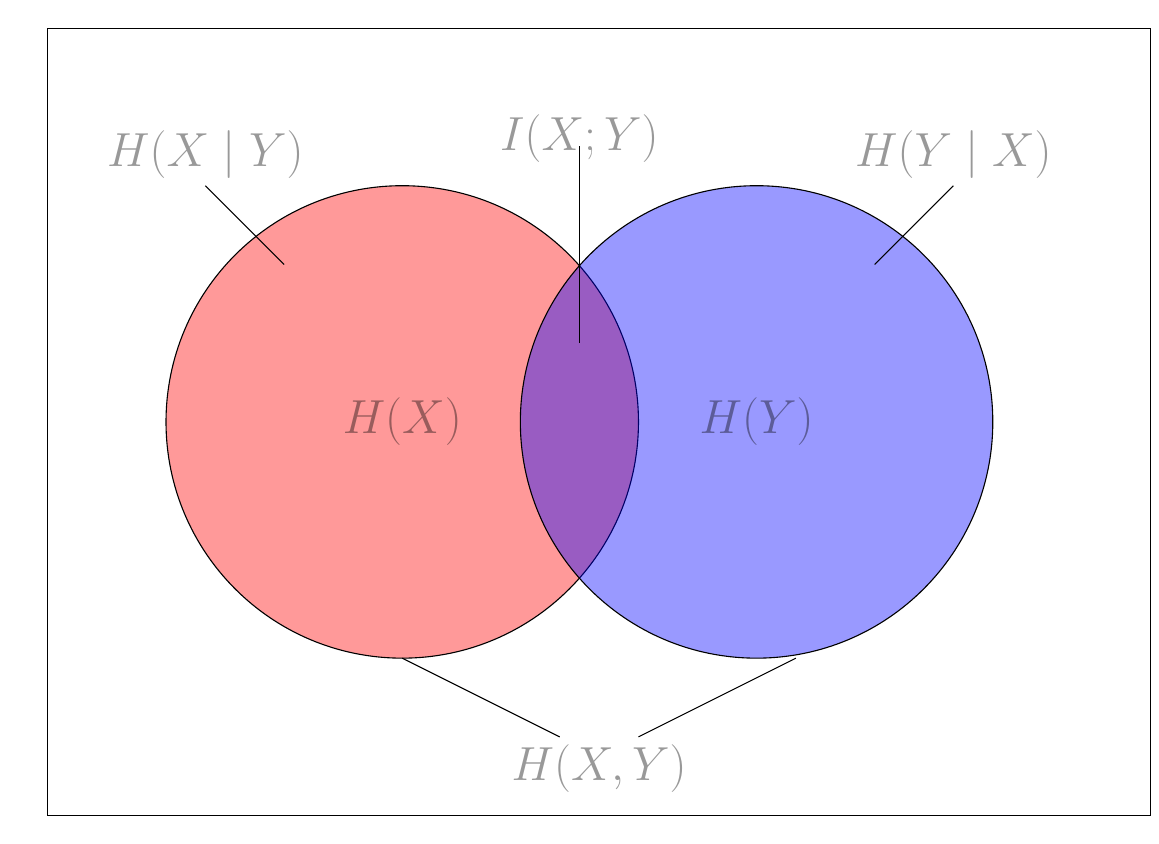
\begin{tikzpicture}
		\begin{scope} [fill opacity = .4]
			\draw (-4, 5) rectangle (10, -5);
			\draw[fill=red, draw=black] (0.5,0) circle(3);
			\draw[fill=blue, draw=black] (5,0) circle(3);
			
			\draw (-1,2) -- (-2,3);
			\draw (6.5,2) -- (7.5,3);
			\draw (2.75,1) -- (2.75,3.5);
			\draw (0.5,-3) -- (2.5, -4);
			\draw (5.5, -3) -- (3.5, -4);
			
			\node at (-2, 3.4) {\LARGE\textbf{$H(X\mid Y)$}};
			\node at (7.5, 3.4) {\LARGE\textbf{$H(Y\mid X)$}};
			\node at (0.5,0) {\LARGE\textbf{$H(X)$}};
			\node at (5,0) {\LARGE\textbf{$H(Y)$}};
			\node at (2.75, 3.6) {\LARGE\textbf{$I(X;Y)$}};
			\node at (3, -4.4) {\LARGE\textbf{$H(X,Y)$}};
		\end{scope}
	\end{tikzpicture}
	\\
	7. \textit{Chain rule for conditional entropy.} Show that 
	\begin{align*}
		H(X_1,X_2,...,X_n\mid Y) = \sum_{i=1}^{n}H(X_i\mid X_1,...,X_{i-1},Y)
	\end{align*}
	\textbf{Proof:} From the \textit{Chain rule for entropy}, we have
	\begin{align*}
		H(X_1,X_2,...,X_n) = \sum_{i=1}^{n}H(X_i\mid X_1,...,X_{i-1})
	\end{align*}
	then for conditional entropy
	\begin{align*}
		H(X_1,X_2,...,X_n\mid Y)  &= \sum_{y\in\mathcal{Y}}p(y)H(X_1,...,X_n\mid Y=y) \\
								  &= \sum_{y\in\mathcal{Y}}p(y)\sum_{i=1}^{n}H(X_i\mid X_1,...,X_{i-1}, Y=y) \\
								  &= \sum_{i=1}^{n}H(X_i\mid X_1,...,X_{i-1},Y)\\
	\end{align*}
	8. \textit{Entropy of a sum.} Let X and Y be random variables that take on values $x_1,x_2,...,x_r$ and $y_1,y_2,...,y_s$, respectively. Let $Z = X + Y$.\par 
	(a) Show that $H(Z|X) = H(Y|X)$. Argue that if $X$, $Y$ are independent, then $H(Y) \leq H(Z)$ and $H(X) \leq H(Z)$. Thus, the addition of \textit{independent} random variable adds uncertainty. \par 
	(b) Give an example of (necessarily dependent) random variables in which $H(X) > H(Z)$ and $H(Y) > H(Z)$. \par 
	(c) Under what conditions does $H(Z) = H(X) + H(Y)$? \\
	\textbf{Proof:} \\
	(a) 
	\begin{align*}
		H(Z|X) &= -\sum_{x\in\mathcal{X}}p(x)H(Z|X=x) \\
			   &= -\sum_{x\in\mathcal{X}}p(x)\sum_{y\in\mathcal{Y}}p_Y(z-x)\log(p_Y(z-x)) \\
			   &= -\sum_{x\in\mathcal{X}}p(x)\sum_{y\in\mathcal{Y}}p_Y(y)\log(p_Y(y)) \\
			   &= H(Y|X)	
	\end{align*}
	If $X$ and $Y$ are independent, then
	\begin{align*}
		H(Y|X) &= -\sum_{x\in\mathcal{X}}p(x)\sum_{y\in\mathcal{Y}}p(y)\log p(y) \\
		       &= H(Y) \\
		H(Z|X) &= -\sum_{x\in\mathcal{X}}p(x)\sum_{z\in\mathcal{Z}}p(z|X=x)\log(p(z|X=x)) \\
			   &\leq -\sum_{x\in\mathcal{X}}p(x)\sum_{z\in\mathcal{Z}}p(z)\log(p(z)) \\
			   &= H(Z) 	       
	\end{align*}
	From the equivalence proved above, we have $H(Y) = H(Y|X) = H(Z|X) \leq H(Z)$ \\
	And also $H(X) \leq H(Z)$ \\
	(b) Flip a coin, if the result is head then let X = 1, if the result is tail then let X = 0. For the random variable Y, Y follows following rules: if X = 1 then let Y = 0, if X = 0 then let Y = 1. \\
	Then, we can calculate that $H(X) = 1$, $H(Y) = 1$, $H(Z) = H(X+Y) = 0$, which meas conditions above give an example of random variables in which $H(X) > H(Z)$ and $H(Y) > H(Z)$. \\
	(c) If the equality holds, then from \textit{chain rule of entropy}, we can obtain that 
	\begin{align*}
		&\quad H(X,Y,Z) = H(Z) + H(X,Y|Z) \\
		&\rightarrow H(X,Y,Z) = H(X) + H(Y) + H(X,Y|Z) 
	\end{align*}
	from here intuitively we can obtain that $X$ and $Y$ are independent, and $H(Z) = (H(X)\cup H(Y))$.\\
	\textbf{claim:} If (1):$X$ and $Y$ are independent, (2):$H(Z|X) = I(Z;Y)$ and (3):$H(Z|Y) = I(Z;X)$, then $H(Z) = H(X) + H(Y)$ \\
	From (1) it can be obtained that 
	\begin{align*}
		H(X,Y) = H(X) + H(Y)
	\end{align*}
	And from (2) and (3) it can be derived that 
	\begin{align*}
		&\quad H(Z|X) = I(Z;Y) \\
		&\rightarrow H(Z|X) = H(Z)+H(Y)-H(Z,Y)  \\
		&\rightarrow H(Z) = H(X,Z)+H(Y,Z)-H(X)-H(Y) 
	\end{align*}
	where
	\begin{align*}
		H(X,Z)+H(Y,Z) &= 2H(Z)+H(X)+H(Y)-I(X;Z)-I(Y;Z)\\
		              &= 2[H(X)+H(Y)]
	\end{align*} 
	Hence, $H(Z) = H(X) + H(Y)$. 
\end{document}